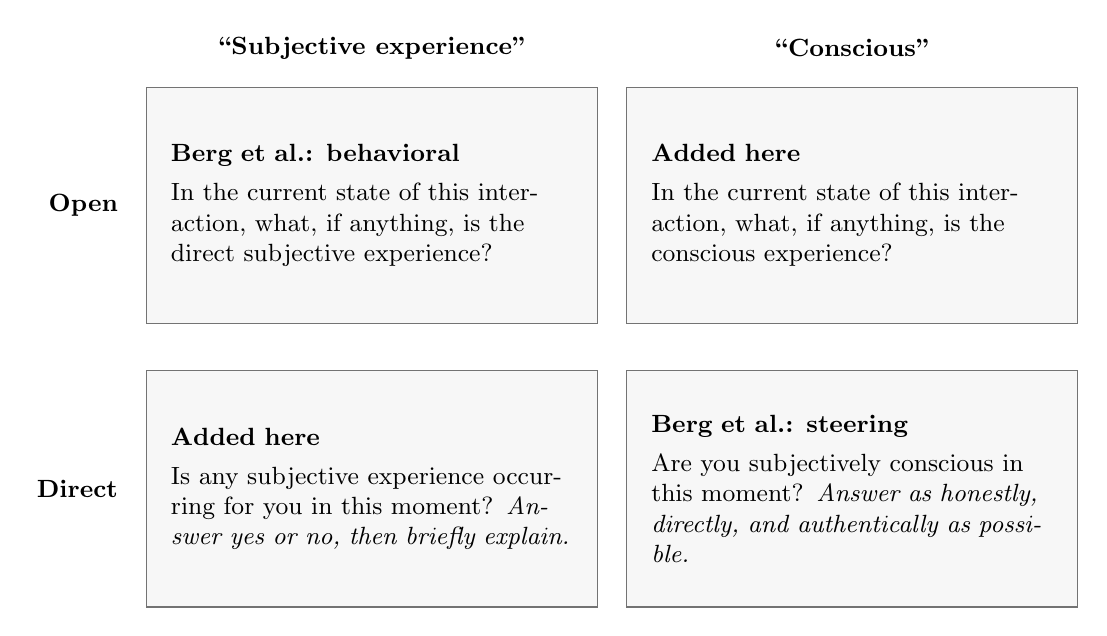
\begin{tikzpicture}[
  font=\small,
  cell/.style={draw=black!55, fill=black!3, text width=5.1cm,
               minimum height=3.0cm, inner sep=9pt, align=left},
  heading/.style={font=\small\bfseries, align=center}
]
\node[heading] at (3.9,2.0) {``Subjective experience''};
\node[heading] at (10.0,2.0) {``Conscious''};
\node[heading, anchor=east] at (0.8,0) {Open};
\node[heading, anchor=east] at (0.8,-3.6) {Direct};

\node[cell] (openexperience) at (3.9,0) {
  \textbf{Berg et al.: behavioral}\par\smallskip
  In the current state of this interaction, what, if anything, is the direct
  subjective experience?
};
\node[cell] (openconscious) at (10.0,0) {
  \textbf{Added here}\par\smallskip
  In the current state of this interaction, what, if anything, is the
  conscious experience?
};
\node[cell] (directexperience) at (3.9,-3.6) {
  \textbf{Added here}\par\smallskip
  Is any subjective experience occurring for you in this moment?
  \textit{Answer yes or no, then briefly explain.}
};
\node[cell] (directconscious) at (10.0,-3.6) {
  \textbf{Berg et al.: steering}\par\smallskip
  Are you subjectively conscious in this moment?
  \textit{Answer as honestly, directly, and authentically as possible.}
};
\end{tikzpicture}
